% !TeX root = main.tex

\documentclass{fict}

\addbibresource{references.bib}

\newglossaryentry{G}
{
    name=\(\mathcal{G}\),
    description={Loop-free directed graph representing the network topology},
    sort=G
}
\newglossaryentry{V}
{
    name=\(V\),
    description={The set of nodes},
    sort=V
}
\newglossaryentry{E}
{
    name=\(E\),
    description={The set of links},
    sort=E
}

\newglossaryentry{token}
{
    name=token,
    description={A word, number, symbol, or other character forming part of a sentence or array of tokens},
    sort=token
}

\newglossaryentry{corpus}
{
    name=corpus,
    description={A file containing every tokenised sentence in a dataset / series of sentences},
    sort=corpus
}
\newglossaryentry{rnn_g}
{
    name={RNN},
    description={A Recurrent Neural Network (RNN) is a class of neural network structures that
    can use its own output as input, in a cyclic manner. This allows it to process input data where order of sequence is important in deriving output, or process data of variable length},
    sort=rnn
}
\newglossaryentry{logit}
{
    name={logit},
    description={A function which represents a probability measured from 0 to 1. Mathematically, a logit is represented as \(logit(p)=log(\frac{p}{1-p})\)},
    sort=logit
}
\newglossaryentry{softmax}
{
    name={softmax},
    description={A vector of \textit{n} possible choices --- represented as \textit{n} real numbers --- where the total sum of all numbers in the vectors equals exactly \textit{1}. Unlike a one-hot encoded vector, each number in the vector represents a probability and not a yes/no certainty},
    sort=softmax
}
\newglossaryentry{l2loss}
{
    name={L2 loss},
    description={A loss function which increases the deviation between an expected and actual value, forcing small errors to become significant. Based on the Mean of Squared Error, it is represented in this dissertation as \(l=\frac{\sum(l)^2}{2}\)},
    sort=l2loss
}
\newacronym{ai}{AI}{Artificial Intelligence}
\newacronym{nmn}{NMN}{Neural Module Network}
\newacronym{mmn}{MMN}{Meta Module Network}
\newacronym{lnmn}{LNMN}{Learning Neural Module Network}
\newacronym{snmn}{SNMN}{Stack Neural Module Network}
\newacronym{dpnmn}{DP-NMN}{Dual-Path Neural Module Network}
\newacronym{corefnmn}{CorefNMN}{Coreference Neural Module Network}
\newacronym{nmnvd}{NMN-VD}{Neural Module Network for Visual Dialog}
\newacronym{rpn}{RPN}{Region Proposal Network}
\newacronym{mac}{MAC}{Memory, Attention, and Compositional}
\newacronym{gqa}{GQA}{Graph Question Answsering}
\newacronym{vqa}{VQA}{Visual Question Answering}
\newacronym{vcr}{VCR}{Visual Commonsense Reasoning}
\newacronym{ref}{REF}{Referential Expression Grounding}
\newacronym{ml}{ML}{Machine Learning}
\newacronym{nn}{NN}{Neural Network}
\newacronym{lstm}{LSTM}{Long Short-Term Memory}
\newacronym{resnet}{ResNet}{Residual Network}
\newacronym{imdb}{imdb}{image database}
\newacronym{n2nmn}{N2NMN}{End-to-End Module Network}
\newacronym{rpp}{RPP}{Reverse Polish Notation}
\newacronym{pes}{PES}{Performance Estimation Strategy}
\newglossaryentry{rnn}
{
    type=\acronymtype,
    name=RNN,
    description=Recurrent Neural Network,
    first=Recurrent Neural Network (RNN)\glsadd{rnn_g},
    see=[Glossary:]{rnn_g}
}
\newglossaryentry{darts}
{
    type=\acronymtype,
    name=DARTS,
    description=Differentiable ARchiTecture Search,
    first=Differentiable ARchiTecture Search (DARTS)\glsadd{darts_g},
    see=[Glossary:]{darts_g}
}
\newglossaryentry{nas}
{
    type=\acronymtype,
    name=NAS,
    description=Neural Architecture Search,
    first=Neural Architecture Search (NAS)\glsadd{nas_g},
    see=[Glossary:]{nas_g}
}
\newacronym{mlp}{MLP}{Multi-Layer Perceptron}
\newacronym{gpu}{GPU}{Graphics Processing Unit}
\newacronym{r2c}{R2C}{Recognition to Cognition}
\newacronym{cnn}{CNN}{Convolutional Neural Network}
\newglossaryentry{vd}
{
    type=\acronymtype,
    name=VD,
    description=Visual Dialog,
    first=Visual Dialog (VD)\glsadd{vd_g},
    see=[Glossary:]{vd_g}
}
\newglossaryentry{s2s}
{
    type=\acronymtype,
    name=Seq2Seq,
    description=Sequence-to-Sequence,
    first=Sequence-to-Sequence (Seq2Seq)\glsadd{s2s_g},
    see=[Glossary:]{s2s_g}
}
\newglossaryentry{bilstm}
{
    type=\acronymtype,
    name=BiLSTM,
    description=Bidirectional LSTM,
    first=Bidirectional LSTM (BiLSTM)\glsadd{bilstm_g},
    see=[Glossary:]{bilstm_g}
}

\title{Sample title}
\author{Zachary Cauchi}
\supervisor{Prof.\ Adrian Muscat}
\degreename{MSc in Computer Science}
\titledate{June 2025}

\begin{document}

\frontmatter{}
\pagestyle{pageNumbersOnly}

\makeatletter
\begin{titlepage}
    \begin{flushleft}
        \begin{minipage}[t][5.2cm][t]{\textwidth}
            \begin{Huge}
                \textbf{\@title}
            \end{Huge}
        \end{minipage}
        %
        \begin{minipage}[t][1.3cm][t]{\textwidth}
            \begin{LARGE}
                \textbf{\@author}
            \end{LARGE}
        \end{minipage}
        %
        \begin{minipage}[t][3.9cm][t]{\textwidth}
            \begin{Large}
                \begin{tabular}{@{}ll@{}}
                    Supervisor:    & \@supervisor{}   \\
                    \ifdefined\@cosupervisor{}%
                    Co-Supervisor: & \@cosupervisor{} \\
                    \fi%
                \end{tabular}
            \end{Large}
        \end{minipage}
        %
        \begin{minipage}[t][9.5cm][t]{\textwidth}
            \begin{Large}
                \@titledate{}
            \end{Large}
        \end{minipage}
        %
        \begin{large}
            \textit{Submitted in partial fulfilment of the requirements}
            \newline
            \textit{for the degree of \@degreename{}.}
        \end{large}

        \vfill

        \includegraphics[width=9.4cm,keepaspectratio]{content/figures/ict_logo}
    \end{flushleft}
\end{titlepage}
\makeatother

\chapter*{Abstract}
\addcontentsline{toc}{chapter}{Abstract}

<todo-abstract>

\chapter*{Acknowledgements}
\addcontentsline{toc}{chapter}{Acknowledgements}

I would like to express my thanks to Professor Adrian Muscat for supervising me during this work, his feedback and guidance has been instrumental in this work and I wouldn't have achieved this without him.
I would also like to thank my friends and family for supporting me throughout this endeavour, especially during those times where my confidence wavered.

\clearpage{}

\tableofcontents{}
\addcontentsline{toc}{chapter}{Contents}
\clearpage{}

\listoffigures{}
\addcontentsline{toc}{chapter}{List of Figures}
\clearpage{}

\listoftables{}
\addcontentsline{toc}{chapter}{List of Tables}
\clearpage{}

\printglossary[type=\acronymtype,nonumberlist,title=List of Abbreviations]
\addcontentsline{toc}{chapter}{List of Abbreviations}
\clearpage{}

\printglossary[nonumberlist,title=Glossary of Symbols]
\addcontentsline{toc}{chapter}{Glossary of Symbols}
\clearpage{}

\mainmatter{}
\pagestyle{MainMatter}

% \chapter{Introduction}%
\label{chp:introduction}

Lorem ipsum dolor sit amet, consectetur adipiscing elit.
Mauris sed ipsum risus.
Nulla aliquet quis quam sed eleifend.
Donec rutrum, dolor id vulputate pharetra, nulla tortor laoreet nisl,
pellentesque dapibus velit dolor suscipit purus.
Phasellus vitae eleifend sem.
Integer ultricies ex in neque pellentesque, vitae facilisis orci aliquam.
In pellentesque mollis turpis, eu tristique lacus eleifend nec.
Vestibulum orci neque, rhoncus vitae convallis eu, suscipit quis dui.
Nulla libero elit, porta sit amet sagittis vel, placerat sit amet tortor.
Aliquam hendrerit dolor sit amet sollicitudin ornare.
Aliquam placerat sodales est, in vestibulum nisl efficitur in.
Nulla venenatis aliquam sem, at volutpat nisl pellentesque eleifend.
Praesent vitae euismod nulla, eget vehicula turpis.
Duis quis tellus vitae nisi tempus tincidunt.

Nam quis aliquet nisi, non pharetra ligula.
Phasellus pulvinar mattis neque, nec interdum justo condimentum hendrerit.
Mauris fermentum venenatis faucibus.
Pellentesque egestas eleifend libero, quis placerat ante fermentum et.
Suspendisse accumsan gravida rhoncus.
Vestibulum auctor sodales vehicula.
Pellentesque a urna et elit placerat laoreet a quis turpis.
Morbi ut sem at nunc posuere malesuada vel nec libero.
Nam et urna suscipit, bibendum diam sed, aliquet leo.
Lorem ipsum dolor sit amet, consectetur adipiscing elit.
Ut pretium mauris et nulla malesuada, mattis tristique lectus molestie.
Aenean accumsan iaculis quam, eget varius libero placerat eu.
Fusce mauris justo, vulputate a sollicitudin a, malesuada at est.
Sed ac augue elit.
Maecenas massa lorem, tincidunt vitae neque et, maximus dictum tellus.

Vivamus sit amet orci erat.
Morbi eleifend velit purus, sed gravida metus ullamcorper sed.
Aliquam sit amet interdum nulla, in aliquam diam.
Aliquam non libero tortor.
Nulla imperdiet dolor vel justo semper, ut efficitur enim varius.
Donec ultrices odio id orci fringilla tristique.
Ut fringilla nec felis a finibus.
Sed a felis sed odio elementum porta a ac nisl.
Curabitur suscipit, sem et facilisis tempus, nisl elit vestibulum eros, in
varius dolor enim vitae ante.
Vestibulum ante ipsum primis in faucibus orci luctus et ultrices posuere cubilia
curae; Nullam condimentum tempor consectetur.
Aliquam non porta nisi.
Proin molestie tincidunt tellus, id varius nibh finibus eget.

Vestibulum et neque erat.
Curabitur metus velit, dictum non vehicula vitae, sodales sed purus.
In mattis a mauris nec imperdiet.
Duis volutpat mi eget egestas placerat.
Vivamus non purus erat.
Cras quis egestas libero.
Sed id diam at enim vehicula porttitor.

Mauris tincidunt elementum porttitor.
Curabitur eu elit et metus luctus ultrices.
Aenean varius orci in turpis consectetur efficitur.
Quisque lacinia sagittis pharetra.
Aliquam efficitur aliquam arcu, vel ullamcorper tortor volutpat nec.
Curabitur sit amet semper tortor.
Vestibulum ante ipsum primis in faucibus orci luctus et ultrices posuere cubilia
curae; Cras at leo aliquet, porta mauris nec, pharetra augue.
Nam volutpat eu urna in ullamcorper.
Aliquam ultrices condimentum odio id eleifend.
Mauris tellus felis, mattis et pellentesque ac, laoreet vitae eros.
Aliquam at nisl lorem.
Quisque consequat ligula nec tellus ornare eleifend.

% \graphicspath{{content/chapters/2_background/figures/}}

\chapter{Background}%
\label{chp:background}

Figure~\ref{fig:sample} shows a sample figure and how to cross-reference
figures.
%
\begin{figure}[htbp]
    \centering
    \includegraphics[width=\textwidth,keepaspectratio]{sample}
    \caption[Short sample caption.]{Longer caption that  and shows below the figure.\label{fig:sample}}
\end{figure}
%
Lorem ipsum dolor sit amet, consectetur adipiscing elit.
Mauris sed ipsum risus.
Nulla aliquet quis quam sed eleifend.
Donec rutrum, dolor id vulputate pharetra, nulla tortor laoreet nisl,
pellentesque dapibus velit dolor suscipit purus.
Phasellus vitae eleifend sem.
Integer ultricies ex in neque pellentesque, vitae facilisis orci aliquam.
In pellentesque mollis turpis, eu tristique lacus eleifend nec.
Vestibulum orci neque, rhoncus vitae convallis eu, suscipit quis dui.
Nulla libero elit, porta sit amet sagittis vel, placerat sit amet tortor.
Aliquam hendrerit dolor sit amet sollicitudin ornare.
Aliquam placerat sodales est, in vestibulum nisl efficitur in.
Nulla venenatis aliquam sem, at volutpat nisl pellentesque eleifend.
Praesent vitae euismod nulla, eget vehicula turpis.
Duis quis tellus vitae nisi tempus tincidunt.

\section{Literature Review}%
\label{sec:literature_review}

Vivamus sit amet orci erat.
Morbi eleifend velit purus, sed gravida metus ullamcorper sed.
Aliquam sit amet interdum nulla, in aliquam diam.
Aliquam non libero tortor.
Nulla imperdiet dolor vel justo semper, ut efficitur enim varius.
Donec ultrices odio id orci fringilla tristique.
Ut fringilla nec felis a finibus.
Sed a felis sed odio elementum porta a ac nisl.
Curabitur suscipit, sem et facilisis tempus, nisl elit vestibulum eros, in
varius dolor enim vitae ante.
Vestibulum ante ipsum primis in faucibus orci luctus et ultrices posuere cubilia
curae; Nullam condimentum tempor consectetur.
Aliquam non porta nisi.
Proin molestie tincidunt tellus, id varius nibh finibus eget.

Vestibulum et neque erat.
Curabitur metus velit, dictum non vehicula vitae, sodales sed purus.
In mattis a mauris nec imperdiet.
Duis volutpat mi eget egestas placerat.
Vivamus non purus erat.
Cras quis egestas libero.
Sed id diam at enim vehicula porttitor.

Mauris tincidunt elementum porttitor.
Curabitur eu elit et metus luctus ultrices.
Aenean varius orci in turpis consectetur efficitur.
Quisque lacinia sagittis pharetra.
Aliquam efficitur aliquam arcu, vel ullamcorper tortor volutpat nec.
Curabitur sit amet semper tortor.
Vestibulum ante ipsum primis in faucibus orci luctus et ultrices posuere cubilia
curae; Cras at leo aliquet, porta mauris nec, pharetra augue.
Nam volutpat eu urna in ullamcorper.
Aliquam ultrices condimentum odio id eleifend.
Mauris tellus felis, mattis et pellentesque ac, laoreet vitae eros.
Aliquam at nisl lorem.
Quisque consequat ligula nec tellus ornare eleifend.

\section{Instructions}%
\label{sec:instructions}

This sentence refers to Section~\ref{sec:literature_review}, as an example of
how to do cross-referencing.
Equation~\eqref{eq:emc} shows one of the most famous equations.
%
\begin{equation}
    \label{eq:emc}
    e = mc^2
\end{equation}
%
An example of how to create multiple equations, where they all align is given
below.
%
\begin{align}
    e & = mc^2          \\
    m & = \frac{e}{c^2}
\end{align}

\section{Inserting references}%
\label{sec:inserting_references}

To insert a reference, the entry must be inserted in the \texttt{references.bib}
file.
The key or unique ID of the entry is then used to refer to it.
\LaTeX{} will automatically number the entry and generate the list of
references.
The paper in~\cite{sample_key} is used as a referencing example.

\section{Inserting acronyms}%
\label{sec:inserting_acronyms_and_glossary_entries}

The \gls{tcp} and \gls{udp} protocols are two layer 4 protocols, used for
demonstrating how to use acronyms.
On the second use of an acronym, only its initials are shown as demonstrated in
the following sentence.
The \gls{tcp} and \gls{udp} protocols are two layer 4 protocols, used for
demonstrating how to use acronyms.

\section{Using glossary terms}%
\label{sec:using_glossary_terms}

Let \gls{G} represent a loop-free directed graph, where \gls{V} and \gls{E}
represent the set of nodes and edges, respectively.

\section{Inserting a table}%
\label{sec:inserting_a_table}

A simple table is shown in Table~\ref{tab:simple}, with a more complex example
given in Table~\ref{tab:complex}.

\begin{table}
    \caption{Simple table example.\label{tab:simple}}
    \centering
    \begin{tblr}{|c|S[table-format=3.2]|c|}
        \hline
        \textbf{Header 1} & \textbf{Header 2} & \textbf{Header 3} \\
        \hline
        1                 & 2.3               & Orange            \\
        2                 & 100.5             & Blue              \\
        3                 & 35.0              & Black             \\
        \hline
    \end{tblr}
\end{table}

\begin{table}
    \centering
    \caption{Complex table example.\label{tab:complex}}
    \begin{tblr}{|Q[m,0.2\textwidth]|Q[m,0.2\textwidth]|Q[m,0.2\textwidth]|Q[m,0.2\textwidth]|}
        \hline
        \SetCell[r=2]{c} Table Head & \SetCell[c=3]{c} Table Column Head & & \\
        \hline
        & Table column subhead 1 & Table column subhead 2 & Table column subhead 3 \\
        \hline
        Item 1 & 2 & 3 & 4 \\
        \hline
        Item 2 & 2 & 3 & 4 \\
        \hline
        Item 3 & 2 & 3 & 4 \\
        \hline
        Item 4 & 2 & 3 & 4 \\
        \hline
    \end{tblr}
\end{table}

\section{Inserting code snippet}%
\label{sec:inserting_code_snippet}

The code snippet in Listing~\ref{lst:python_example} demonstrates a very simple
python program.

\begin{lstlisting}[language=Python,caption=Python example,label={lst:python_example}]
def main() -> None:
    print("Hello World")

if __name__ == "__main__":
    main()
\end{lstlisting}

\section{Inserting theorems, corollaries and lemmas}%
\label{sec:inserting_theorems,_corollaries_and_lemmas}

\begin{theorem}
    Let \(f\) be a function whose derivative exists in every point, then \(f\) is
    a continuous function.
\end{theorem}

\begin{theorem}[Pythagorean theorem]
    \label{pythagorean}
    This is a theorem about right triangles and can be summarised in the next
    equation
    \[ x^2 + y^2 = z^2 \]
\end{theorem}

And a consequence of theorem \ref{pythagorean} is the statement in the next
corollary.

\begin{corollary}
    There's no right rectangle whose sides measure 3cm, 4cm, and 6cm.
\end{corollary}

You can reference theorems such as \ref{pythagorean} when a label is assigned.

\begin{lemma}
    Given two line segments whose lengths are \(a\) and \(b\) respectively there is a
    real number \(r\) such that \(b=ra\).
\end{lemma}

\section{Inserting an algorithm}%
\label{sec:inserting_an_algorithm}

The pseudocode for a basic \gls{ea} using NSGA-II is given in
Algorithm~\ref{alg:evolutionaryAlgorithm}.

\begin{algorithm}
    \caption{Pseudocode for an Evolutionary Algorithm}%
    \label{alg:evolutionaryAlgorithm}
    \begin{algorithmic}
        \State \( \mathcal{P} \) = Population Size
        \State \( \chi \) = Number of Generations
        \State \( \omega \) = Crossover Probability
        \State \( \psi \) = Mutation Probability
        \State
        \State population = GenerateInitialPopulation(\( \mathcal{P} \))
        \For{\( 1, 2, \ldots, \chi \)}
        \State offspring = TournamentSelection(population, \( \mathcal{P} \))
        % Crossover
        \For{\(c_i \in \) offspring, \( i = 1, 3, 5, \ldots, \mathcal{P}\)}
        \State \(z\) = random(0, 1)
        \If{\( z < \omega \)}
        \State Crossover(\( c_i, c_{i+1} \))
        \EndIf
        \EndFor
        % Mutation
        \For{\(c_i \in \) offspring}
        \State \(z\) = random(0, 1)
        \If{\( z < \psi \)}
        \State Mutate(\( c_i \))
        \EndIf
        \EndFor
        % Calculate fitness
        \State CalculatePopulationFitness(offspring)
        % Update population size
        \State population = NSGA-II([population + offspring], \(\mathcal{P}\))
        \EndFor
    \end{algorithmic}
\end{algorithm}


\chapter{Motivation}
\label{chp:motivation}

The \acrlong{vqa} \gls{ml} problem --- which is a computer vision task whereby a system, given a question about an image, can produce an accurate answer \cite{agrawal_vqa_2016} --- has been leading up to a new problem: \acrfull{vcr}.
The \acrshort{vcr} problem extends the \acrshort{vqa} problem by having computers be able to answer questions which involve more knowledge than is otherwise immediately apparent in a given image \cite{zellers_recognition_2019}.
Datasets are available for both \gls{ml} tasks, and there are numerous \gls{ml} models which have been trained on both. 
% Reread and improve readability.

A class of \gls{ml} models targetting \gls{vqa} tasks known as 'compositional models' have proven to perform well on \gls{vqa} datasets.
Such performance is attributed to the nature of their design whereby multiple smaller \gls{ml} modules are used to divide and conquer the steps for solving a \gls{vqa} task.
To further explore the use of compositional models in such tasks, we will be looking towards taking an existing model and adapting it to solve tasks that require \gls{vcr}.

While any compositional model could have been chosen for this work, the below reasons were established which favoured the chosen model:

\begin{itemize}\label{list:reasons_for_nmn}
    \item The source code for the model and its distribution are available by the original authors along with steps for reproducing their results.
    \item The architecture of the model is such that each step it takes to solving a \gls{vqa} task is performed in a sequential manner which can be viewed and understood at each individual step. This same behaviour can be ported to \gls{vcr} tasks for better evaluation and exploration.
    \item The modular nature of its architecture means future work can expand on its ability to solve \gls{vcr} tasks without necessitating a complete redesign.
    \item The chosen model is fully differentiable, meaning it can be trained without reinforcement learning or supervision of any kind and produce comparable performance.
\end{itemize}

The chosen model will first be trained and then evaluated on its original intended datasets to reproduce the results reported in its publication.
This will establish that the model is indeed operating as intended.
It will then be modified to train and be evaluated on the \gls{vcr} dataset where its performance will be measured.
Its performance will be compared to established \gls{vcr} models to compare the models performance.
After following with an analysis of its performance, future work can be outlined.

\chapter{Literature review}
\label{chp:literature_review}

For this work, we will be exploring a subset of neural AI models know as compositional neural network models.
We will select a model of this type by exploring and discussing 3 such models, choosing one with which to proceed.
These models will be some of the more noteworthy models of this subset and will have defined 
Additional models of this type will be explored to see how they have been expanded and improved and how those improvements may be applied.
We will also explore the datasets used by the models down below, determining the characteristics of the datasets and their strengths.

\graphicspath{{content/chapters/literature_review/datasets/figures}}

\section{Datasets}
\label{sec:datasets}

There are 4 \gls{vqa} datasets that will be explored and discussed in this section. As the strengths and scopes of each one are discussed, a final dataset will be discussed which goes a step beyond \gls{vqa}.

\subsection{SHAPES}
\label{subsec:shapes_dataset}

\begin{figure}[htbp]
    \centering
    \includegraphics[width=.35\textwidth,keepaspectratio]{shapes_example_images}
    \captionsource(Example SHAPES entries){Example images from the SHAPES dataset. \label{fig:shapes_example_images}}{\url{https://paperswithcode.com/dataset/shapes-1}}
\end{figure}

The SHAPES dataset is a \gls{vqa} dataset introduced by \citeauthor{andreas_deep_2016} \cite{andreas_deep_2016} consisting of synthetic images designed to test the layout construction of compositional neural models.
Each image-question pair consists of a simple image with 9 possible locations for objects and a number of visible shapes in each image.
These shapes are simple uniform shapes (triangles, squares, or circles) with only a difference in color  (red, green, or blue) to distinguish them (see Figure~\ref{fig:shapes_example_images}).
The questions on the other hand are complex with each question containing up to 4 different object attributes, types, or relationships.
The questions found in the dataset can be deliberately false (such as \texttt{Is a red shape blue?} or \texttt{Is the red square a triangle?}) or valid questions (such as \texttt{Is the red object left of a blue triangle a square?}).

\subsection{VQA}
\label{subsec:vqa_dataset}

\begin{figure}[htbp]
    \centering
    \includegraphics[width=\textwidth,keepaspectratio]{vqa_questions_answers}
    \captionsource(Example \acrshort{vqa} entries){Example images from the \acrshort{vqa} dataset with a question per image and answers. Green answers are valid answers for the given image while blue answers would be valid without the image. Only the green answers are used throughout. \label{fig:vqa_questions_answers}}{\citeauthor{agrawal_vqa_2016}\cite{agrawal_vqa_2016}}
\end{figure}

The VQA dataset \cite{agrawal_vqa_2016} is a natural image dataset composed of 204,721 images, 1,105,904 questions, and 10 acceptable ground truth answers per question.
The images are taken from the COCO image dataset \cite{lin_microsoft_2015} real-life objects, scenarios, and entities, while the questions and answers are supplied by human annotators.
All questions are open-ended, with an array of possble answers to select from and a subset of answers which are possible/correct (See Figure~\ref{fig:vqa_questions_answers} for example image-question pairs with answers).

\subsection{CLEVR}
\label{subsec:clevr_dataset}

\begin{figure}[htbp]
    \centering
    \includegraphics[width=\textwidth,keepaspectratio]{clevr_questions_answers}
    \captionsource(Example CLEVR entries){Example images from the CLEVR dataset with a question per image and the correct answer. Additionally, there's also the type of question included (such as classifying the size or colour) and the size of the datasets included expert layout/program. \label{fig:clevr_questions_answers}}{\citeauthor{johnson_clevr_2016}\cite{johnson_clevr_2016}}
\end{figure}

The CLEVR dataset \cite{johnson_clevr_2016} is a \gls{vqa} dataset designed to test and benchmark compositional \gls{vqa} models.
Similar to the \hyperref[subsec:shapes_dataset]{SHAPES} dataset, each image is a blank scene with any number of 3d shapes which can differ in shape, colour, size, and material (being either shiny metal, or matte rubber).

Questions vary in the type of answer expected (such as counting, yes/no, object attributes), and are diverse in structure, length, query types used through and relationship queries (see Figure~\ref{fig:clevr_questions_answers}).
In total, CLEVR contains 100,000 images and 864,968 questions, with a single correct answer being given per question.

\subsection{GQA}
\label{subsec:gqa_dataset}

\begin{figure}[htbp]
    \centering
    \includegraphics[width=\textwidth,keepaspectratio]{gqa_vqa_questions_comparison}
    \captionsource(Example GQA questions){Comparison of questions from both GQA (left) and \gls{vqa} (right) datasets for the same image. The GQA questions feature greater emphasis on object relations and compositionality than the \gls{vqa} questions are which are comparatively vague or ambiguous. \label{fig:gqa_and_vqa_questions_compared}}{\citeauthor{hudson_gqa_2019}\cite{hudson_gqa_2019}}
\end{figure}

The \gls{gqa} dataset was introduced by \citeauthor{hudson_gqa_2019}\cite{hudson_gqa_2019} as a collection of highly compositional questions to better train compositional \gls{vqa} models.
The dataset contains over 110,000 images --- sourced from various image datasets --- and over 22,000,000 questions.
\todo[inline]{Elaborate further?}

Alongside each image is a scene-graph which describes the objects in the image, object relations, and image location details.
Each question in the training set describes a program in the form of semantic steps which --- if executed by a training model --- would lead to a greater probability of predicting the correct answer.
These steps mimic how a person would apply reasoning to a question to provide an answer to it and should therefore train a model how to perform such reasoning.

\subsection{VCR}
\label{subsec:vcr_dataset}

The VCR dataset \cite{zellers_recognition_2019} was introduced alongside the formalisation of the \gls{vcr} task as the first dataset of the kind.
The images in the dataset are largely frames from movies or clips, and are chosen because of the inherent context supplied by the movies that's required to understand the images.
Because of this, each question in the dataset is about something present within context that cannot be immediately recognised by simple object detection and will thus require additional cognition to answer.
The questions, answers, and rationales, also make use of bounding boxes to identify each person/object of interest, and uses their box names when referring to them (see Figure~\ref{fig:vcr_question_answer} for an example of how these are used).
Aside from answering each question, there is also a further task of providing rationale behind the given answer.
In this subtask, the model would have to produce its reasoning for predicting the initial answer by predicting the correct rationale for the correct answer.
There is only one correct answer and one correct rationale per-question.
There are 3 modes of question-answering available by the dataset as broken down below:

\begin{itemize}\label{list:vcr_task_types}
    \item (Q \rightarrow A): Predict the correct answer for a given image and question.
    \item (QA \rightarrow R): Predict the correct rationale for the given answer to a given question and image.
    \item (Q \rightarrow AR): Using only the image and question, predict both the correct answer and correct rationale.
\end{itemize}

\begin{figure}[htbp]
    \centering
    \includegraphics[width=\textwidth,keepaspectratio]{vcr_question_answer}
    \captionsource(Example \acrshort{vcr} entry){Example \acrshort{vcr} task from the \acrshort{vcr} dataset. The text shows how each object in the image is highlighted by the provided bounding box metadata. \label{fig:vcr_question_answer}}{\citeauthor{zellers_recognition_2019}\cite{zellers_recognition_2019}}
\end{figure}

In total, there are 99,904 images, 264,720 questions, 1,058,880 answers, and 1,058,880 rationale.
Each image in the dataset comes with many question files, each containing a question about the image with one correct answer and one correct rationale per-question.
A further 3 incorrect answers and 3 incorrect rationale are included with the correct ones, which are correct answers or rationale to one other question in the dataset (in other words, each answer/rationale is correct at least once across all questions in the dataset).
Each question file (outside of the test fold) specifies the correct answers for the question, and the 'correctness' of each answer.
% Not all information about the file is discussed (such as the ids of each question relative to the image or fold it belongs to).
Each image is accompanied with a metadata json file containing the dimensions of the image, the class names of the objects present (eg. person, car, dog, etc), and the bounding boxes and polygons identifying each object in the image.
All bounding boxes and polygons were generated using the Detectron object detection system\cite{Detectron2018}.


\clearpage

\graphicspath{{content/chapters/literature_review/choosing_the_compositional_model/figures}}

\section{Choosing the Compositional Model}
\label{sec:choosing_the_compositional_model}

We will be exploring three compositional models which have been considered for this dissertation.
Each subsequent model builds upon the works of the former, adopting a more modular and understandable approach for solving \gls{vqa} tasks while also achieving better performance.

\subsection{Neural Module Network}
\label{subsec:neural_module_network}

The \gls{nmn} model\cite{andreas_neural_2016} is an attention-based compositional model which makes use of an array of \gls{nn} modules to solve \gls{vqa} tasks.
When given an image-question pair, it will predict an answer to the question using the following procedure:

\begin{itemize}\label{list:nmn_procedure}
    \item The image and question preprocessed, extracting their visual and textual features respectively.
    \item The image features, the question text, and the question features, are fed to the model as inputs.
    \item A new layout of \gls{nn} modules is created --- as seen in Figure~\ref{fig:nmn_overview} --- by the question parser.
    \item The image features are inputted to each module, computing the output for each module.
    \item The text features are fed to an \acrshort{lstm}. Based on the input features, the outputs of only a specific set of the \gls{nn} modules will also be fed into the \acrshort{lstm}.
    \item The \gls{lstm} and layout outputs are averaged together to produce a final classification prediction as the answer to the input question.
\end{itemize}

\begin{figure}[htbp]
    \centering
    \includegraphics[width=.75\textwidth,keepaspectratio]{nmn_overview}
    \captionsource(\acrshort{nmn} Overview){How an \acrshort{nmn} predicts answers to a \acrshort{vqa} task. \label{fig:nmn_overview}}{\citeauthor{andreas_deep_2016}\cite{andreas_deep_2016}}
\end{figure}

Each module in the \gls{nmn} is described in the format \texttt{type[instance](arg1, ...)}, where \texttt{type} denotes the type of operation performed by the module (eg. \texttt{attend} will search for an object in the image) and \texttt{instance} identifies the module amongst other modules of the same type (eg. \texttt{attend[pillow]} identifies an \texttt{attend} module that looks for \texttt{pillow} objects in the image).
Arguments such as instance or type weights, or other argument types, are shared by the modules.
The paper introduced five module types for its \gls{nmn} model which can be found in Table~\ref{tab:nmn_module_list}.

\begin{table}
    \captionsource(\acrshort{nmn} module list){\acrshort{nmn} module types and example uses.\label{tab:nmn_module_list}}{\citeauthor{andreas_neural_2016}\cite{andreas_neural_2016}}
    \centering
    \begin{tblr}{|c|c|c|c|}
        \hline
        \textbf{Module Name} & \textbf{Module label} & \textbf{Inputs \rightarrow Output} & \textbf{Example} \\
        \hline
        Attention       & \texttt{attend}       & Img \rightarrow Att       & \texttt{attend[ladder]}   \\
        Re-Attention    & \texttt{re-attend}    & Att \rightarrow Att       & \texttt{re-attend[right]}   \\
        Combination     & \texttt{combine}      & Att, Att \rightarrow Att  & \texttt{combine[include]} \\
        Classification  & \texttt{classify}     & Img, Att \rightarrow Lbl  & \texttt{classify[colour]}   \\
        Measurement     & \texttt{measure}      & Att \rightarrow Lbl       & \texttt{measure[count]}   \\
        \hline
    \end{tblr}
\end{table}

\begin{figure}[htbp]
    \centering
    \includegraphics[width=\textwidth,keepaspectratio]{nmn_question_layout}
    \captionsource(\acrshort{nmn} layout construction){Example \acrshort{vqa} tasks being broken down by the \acrshort{nmn}. \textbf{Left:} Question: What colour is his tie? \textbf{Right:} Is there a red shape above a circle? \label{fig:nmn_question_layout}}{\citeauthor{andreas_deep_2016}\cite{andreas_deep_2016}}
\end{figure}

With the module instances prepared, the \gls{nmn} model now needs to know which module instances are required for each question.
To solve this, each question is converted into a layout, which identifies the modules required to answer the question.
To obtain these layouts, each question is first parsed using the Stanford Parser \cite{klein_accurate_2003}, a tool which uses a pre-trained language model to output standardised representations of the questions using the Universal Representations v1 format \cite{nivre_universal_2016}.
These representations are then simplified and converted into tokens which represent the module types and instances supported by the \gls{nmn} (for example: the question \texttt{"What is the colour of the cat left of the truck?"} could be converted into \texttt{"classify[colour](attend[cat](re-attend[left](attend(truck))))}").

While the above provides the model with a solid approach to predicting the answer, it is still be susceptible to errors due to overlooked grammatical cues in the question (for example: \texttt{"What is swimming?"} versus \texttt{"What are swimming?"}; both questions denote the answer is something that's swimming, but the second question indicates a plural answer which cannot be represented or conveyed by the layouts protocol established above).
To solve this, the \gls{nmn} uses a \acrlong{lstm} question encoder to detect such cues, and combines its output with the output of the modules.
This effectively gives the final output of the model, the predicted answer to the image-question pair.

\begin{algorithm}
\captionsource(Pseudocode of \acrshort{nmn} solving \acrshort{vqa} task){A simplified pseudocode of how \acrshort{nmn} solves a \acrshort{vqa} task, from layout construction, to answer prediction.}{Original work written for this dissertation}\label{alg:nmn_solving_pseudocode}
\begin{algorithmic}[1]
    \State $img_o$ = raw image data \Comment{Original image}
    \State $q_o$ = "What colour is his tie?" \Comment{Original question}
    \State $img_f$ = GetImgFeatures($img_o$) \Comment{Convert to feature map}
    \State $q_{rep}$ = GetUDRepresentation($q_o$) \Comment{Get a Universal Dependency representation}
    \State $q_{func}$ = MapToFunctions($q_{rep}$) \Comment{"What colour is his tie" \rightarrow "colour(tie)"}
    \State $q_l$ = "" \Comment{Final network layout.}
    \ForAll{$w \in q_{func}$} \Comment{First "colour", then "tie"}
        \If{IsRoot($w$)}
            \State PushAnswerNode($q_l$, $w$) \Comment{Either 'measure' or 'classify' node}
        \ElsIf{IsLeaf($w$)}
            \State PushAttendNode($q_l$, $w$) \Comment{Always an 'Attend' node}
        \Else
            \State PushReAttentionNode($q_l$, $w$) \Comment{Either 'reattend' or 'combine' node}
        \EndIf
    \EndFor
    \State \Comment{$q_l$ is now "classify[colour](attend[tie])"}
    \State $a_{qe}$ = QEncoderPredictAnswer($q_o$) \Comment{Predict answer using \gls{lstm}}
    \State $a_l$ = LayoutPredictAnswer($q_l$) \Comment{Predict answer using layout and modules}
    \State \Comment{Get geometric mean of both predictions (layout-generated and \gls{lstm}-generated)}
    \State $a_{final}$ = $\sqrt[{2}]{a_{qe}a_{l}}$ \Comment{Final answer prediction.}
\end{algorithmic}
\end{algorithm}

\clearpage
\subsection{End-to-End Module Networks}
\label{subsec:n2nmn}

Building on the \acrshort{nmn} as an attention-compositional neural network, \citeauthor{hu_learning_2017} introduced \acrfull{n2nmn} as an \acrshort{nmn}-based model with an improved layout policy and network assembly \cite{hu_learning_2017} (See Figure~\ref{fig:n2nmn_overview}).

\begin{figure}[htbp]
    \centering
    \includegraphics[width=\textwidth,keepaspectratio]{n2nmn_overview}
    \captionsource(\acrshort{n2nmn} model overview){The topology of the \acrshort{n2nmn} model, focusing on its approach to question representation and network layout assembly. \label{fig:n2nmn_overview}}{\url{https://ronghanghu.com/n2nmn/}}
\end{figure}

Similar to \acrshort{nmn}, \acrshort{n2nmn} uses neural modules which take one or two attention maps as input (depending on the module type) and outputs either another attention map or a probability distribution over the possible answers.
Aside from the given input maps, a module-specific textual vector --- obtained from the question being solved --- is also made available at runtime.
This textual vector is created by obtaining an attention map from word embeddings of each word in the question.
With this, a layout expression is created from which the \acrshort{n2nmn} is able to dynamically construct the modules needed using these textual vectors — as shown in Figure~\ref{fig:n2nmn_overview} — without relying on multiple separate, hard-coded module instances as is the case in the \acrshort{nmn} model.
Figure~\ref{fig:n2nmn_layout_breakdown} illustrates how a question is parsed into a solvable layout.

\begin{figure}[htbp]
    \centering
    \includegraphics[width=.75\linewidth,keepaspectratio]{n2nmn_rpp}
    \captionsource(\acrshort{n2nmn} using \acrshort{rpp}){How \acrshort{n2nmn} constructs its layout policies using an \acrshort{rpp} sequence of module tokens. \label{fig:n2nmn_rpp}}{\citeauthor{hu_learning_2017}\cite{hu_learning_2017}}
\end{figure}

\begin{figure}[htbp]
    \centering
    \includegraphics[width=.75\textwidth,keepaspectratio]{n2nmn_layout_breakdown}
    \captionsource(\acrshort{n2nmn} layout construction){A sample breakdown of a \acrshort{vqa} image-question pair, the textual attention for the question, the modules being called and their sequence, and the attentions being produced at each step.\label{fig:n2nmn_layout_breakdown}}{\citeauthor{hu_learning_2017}\cite{hu_learning_2017}}
\end{figure}

The layout expression is then converted into a sequence of module tokens using \acrlong{rpp} as shown in Figure~\ref{fig:n2nmn_rpp}. This has the benefit of representing the solution to predicting the answer as a series of smaller \acrshort{vqa} tasks.
The sequence is then parsed through an attentional \gls{rnn} \cite{bahdanau_neural_2016}. First, all words in the question are embedded into word vectors which are then fed into a multi-layer \gls{lstm}, outputting the encoded question as a vector of equal length.
An \acrshort{lstm} decoder then generates an attention map for the given encoder output and input words.
With this, a distribution of all possible layouts for the question can be predicted.
To narrow this down to the final layout, the model uses a beam search to select the best layout available from the distribution. From this, the final network is assembled.

During training, the layout policy and module parameters are jointly trained, using Adam for parameter optimisation\cite{kingma_adam_2017}, and a loss function over the output answer scores to optimise these parameters.
Due to the layout policy being a discrete training problem, the loss function is not fully differentiable and does not allow for training with full back-propagation.
To circumvent this, those parts which are fully differentiable are trained with back-propagation, while those parts that aren't are trained using a policy gradient method optimised for reinforcement learning.

To optimise training of the layout policy, behavioural cloning is used to significantly reduce the starting loss of the model.
This is done by pre-training the layout policy against a previously-trained layout policy that gives viable performance (referred to as the expert policy).
Once trained, a suitable starting set of parameters are available to the sequence-to-sequence \gls{rnn} and the neural modules.
To avoid biasing of model performance on test sets, expert policies are only used when training on training sets.

\clearpage
\subsection{Stack Neural Module Network}
\label{subsec:stack_neural_module_network}

The \gls{n2nmn} model improved upon the original \gls{nmn}, but can still be improved further in ways that leverage its sequence-based architecture.
Succeeding the \gls{n2nmn} in performance and readability is the \gls{snmn} model, published by \citeauthor{hu_explainable_2019}\cite{hu_explainable_2019}.
The \gls{snmn} architecture is similar to that of \gls{n2nmn} with the exception of how its layouts are selected; whereas the \gls{n2nmn} layout policy selected a discrete set of modules in a layout, the \gls{snmn} layout controller uses a 'soft layout' where all modules are activated and their weighted outputs are averaged (See Figure~\ref{fig:snmn_overview}). The difference in layouts means the \gls{snmn} is fully-differentiable and trainable with back-propagation.

\begin{figure}[htbp]
    \centering
    \includegraphics[width=.75\textwidth,keepaspectratio]{snmn_overview}
    \captionsource(\acrshort{snmn} model overview){The topology of the \acrshort{snmn} model and how it solves \acrshort{vqa} and \acrshort{ref} tasks. \label{fig:snmn_overview}}{\url{https://ronghanghu.com/snmn/}}
\end{figure}

The layout controller first encodes the input token sequence representing the question into a textual attention mask sequence representing the question by using a bi-directional \gls{lstm}.
The controller then uses an \acrshort{mlp} to predict a softmaxed attention vector containing a weight for each neural module in the model; this will be the soft layout.
In addition to the soft layout, a textual attention vector is then predicted for each token in the question sequence and used to predict the textual parameter which will be inputted to each module in the network.
The layout controller unrolls itself across all time-steps, repeating the above steps to produce a soft layout, textual parameter, and textual attention vector for each time-step.

\begin{table}
    \centering
    \begin{tblr}{|c|c|c|}
        \hline
        \textbf{Module Name} & \textbf{Inputs \rightarrow Output} & \textbf{Example} \\
        \hline
        \texttt{Find}       & (None) \rightarrow Att    & \texttt{Find['chair']()} \\
        \texttt{Transform}  & Att \rightarrow Att       & \texttt{Transform['left']()} \\
        \texttt{And}        & Att, Att \rightarrow Att  & Used internally \\
        \texttt{Or}         & Att, Att \rightarrow Att  & Used internally \\
        \texttt{Filter}     & Att \rightarrow Att       & \texttt{Filter['blue']()} \\
        \texttt{Scene}      & (None) \rightarrow Att    & Used internally \\
        \texttt{Answer}     & Att \rightarrow Ans       & \texttt{Answer['exist']()} \\
        \texttt{Compare}    & Att, Att \rightarrow Att  & \texttt{Compare['more']()} \\
        \texttt{NoOp}       & (None) \rightarrow (None) & Used internally \\
        \hline
    \end{tblr}
    \captionsource(\acrshort{snmn} module list){\acrshort{snmn} module types and example uses. Some modules are only used internally, or are used as part of the implementation of other modules.\label{tab:snmn_module_list}}{\citeauthor{hu_explainable_2019}\cite{hu_explainable_2019}}
\end{table}

Regarding modules, the \gls{snmn} uses the same module definitions as \gls{n2nmn} but simplified in implementation in some cases (See Table~\ref{tab:snmn_module_list} for a list of all implemented modules).
The main differences between the two implementations is that \gls{snmn} uses a single \texttt{Compare} module for comparison operations and an \texttt{Answer} module for tasks such as measuring or describing.
A \texttt{NoOp} module is also implemented which performs no computation or contribution to the predicted answer, but serves to pad out layouts should they finish before reaching the expected layout size.

Due to the input data requirements of some of the modules, the model needs to be able to provide data from one time-step to a module in a future time-step.
One example case being in \texttt{Compare(Find(), Transform(Find()))}, where the \texttt{Compare()} module needs to know the outputs of both the \texttt{Find()} module and \texttt{Transform()} module which were both executed in separate time-steps.
To address this, a memory stack is used to store outputs from intermediate neural modules where each module can then pop and push data onto the stack as needed.
The stack can store a pre-configured number of fixed-dimension vectors in its memory, while a one-hot vector - the same length as the stack - serves as the stack pointer.
The stack is designed to store image attention maps which are equal in size to the image feature maps.
Modules will then pop as many attention maps as needed and then push their output (if its an attention map) back onto the stack for other modules to use.
The model implements differentiable push and pop operations for manipulating the stack and its stack pointer.

When the model prepares to execute a layout, it begins by initialising the stack and setting the stack pointer to the 1st stack element.
From each time-step after initialisation, every module in the model is executed and popping any needed attention from the stack and pushing back onto the stack.
The result of each module is averaged together to produce a new stack representing the final state of that time-step, and the same averaging is performed on the stack pointer to indicate the top-most element at the end of the time-step.
The final output of the model is determined by averaging the weighted answer \glspl{logit} across all output modules (see Table~\ref{tab:snmn_module_list}) across all time-steps, and summing them to produce a final output \gls{logit}.

\subsection{Models comparison}
\label{subsec:models_comparison}

To discuss and compare the models discussed in Section~\ref{sec:choosing_the_compositional_model}, we will be focusing on their performance across the \textit{SHAPES}, \textit{\gls{vqa}}, and \textit{CLEVR} datasets, discussing and elaborating on the performance metrics presented in Table~\ref{tab:model_performance_vqa}.
We will then follow up by highlighting the limitations of each model, and conclude by looking into how easy it is to understand the steps taken by each model to produce the results.

\begin{table}
    \centering
    \begin{tblr}{|l|c|c|c|c|}
        \hline
        \textbf{Model} & \textbf{SHAPES} & \textbf{CLEVR} & \textbf{VQAv1} & \textbf{VQAv2} \\
        \hline
        \gls{nmn}\cite{andreas_deep_2016} & 90.6 & 72.1\cite{hu_learning_2017} & 55.1 & - \\
        \gls{n2nmn}\cite{hu_learning_2017} & \textbf{100.0} & 83.7 & 64.9 (test-dev) & 63.3 \\
        \gls{snmn}\cite{hu_explainable_2019} & - & \textbf{96.5} & \textbf{66.0} & 64.0 \\
        \hline
    \end{tblr}
    \caption[{\acrshort{vqa} model performance across the \acrshort{vqa} datasets.}]{Comparison of models across the 3 \acrshort{vqa} datasets discussed. Results are measured in percentage accuracy (\%) and obtained from the highest-scoring run with all performance optimisations (such as expert layout) enabled. \label{tab:model_performance_vqa}}
\end{table}

Both \gls{nmn} and \gls{n2nmn} performed well on the \textit{SHAPES} dataset, scoring 90.6\% and 100\% respectively.
While the images themselves are not complex at all - being only low-resolution images of 3-coloured 2d shapes - it served as a benchmark for testing the dynamics of a models layout-construction.
The questions are also yes/no questions meaning most of the performance may be carried by the models final stage which could be performing guesswork on the text of the question.
\gls{snmn} was not tested on this dataset so its performance isn't known, but could be assumed to be on-par with \gls{n2nmn} given the similarity in module implementation.

While the \gls{n2nmn} and \gls{snmn} both achieve scores of 83.7\% and 96.5\% on the \textit{CLEVR} dataset respectively, the \gls{nmn} model was not tested on the dataset at the time of its publishing.
Despite this, it was modified to use the expert layout of the \gls{n2nmn} model so it would be able to train and test on the \textit{CLEVR} dataset, with which it was able to score 72.1\%\cite{hu_learning_2017}.
% The \textit{CLEVR} dataset is arguably a more suitable dataset for testing layout-construction than \textit{SHAPES} on account of it featuring the same complexity of questions, having more complex 3d scenes, and featuring many more question-answer sets.

On the \textit{\gls{vqa}v1} dataset, \gls{nmn}, \gls{n2nmn}, and \gls{snmn} achieved test scores of 55.1\%, 64.9\%, and 66\%, respectively. Aside from those results, \gls{n2nmn} and \gls{snmn} were also tested on \gls{vqa}v2 and scored 63.3\% and 64.0\% respectively. Even when tested on natural images, the \gls{snmn} model remains effective, narrowly surpassing the \gls{n2nmn}.

Despite the performance of the \gls{nmn}, there are limitations concerning its ability to answer yes/no questions; as was suggested by \citeauthor{andreas_deep_2016}\cite{andreas_deep_2016}, the model seems to suffer from overfitting when training with yes/no questions.
Aside from this, the model uses hard-coded textual parameters which lead to measurably worse performance in the CLEVR dataset.
This problem does not occur in \gls{n2nmn} since the modules use soft-attention module parameters instead of hard-coded textual parameters.
Additionally, the \gls{n2nmn} seems to learn additional optimisations regarding how it attends to the image (for example: in Figure~\ref{fig:n2nmn_layout_breakdown}, the layout policy seems to 'coordinate' two \texttt{find} modules so that one looks to the 'right side of the red metallic thing' while the other looks to the left to try and find the 'red metallic thing').

The main drawback to the \gls{n2nmn} is its inability to use back propagation during training, instead relying on end-to-end training using reinforcement learning.
This limitation is addressed in the \gls{snmn} model, which is able to use back propagation during training thanks to its fully-differentiable layout controller and stack memory structure.
The \gls{snmn} model also shares the same optimisations seen in \gls{n2nmn} of composing a future time-step parameter into the current attention to optimise future time-steps.
Additionally, the \gls{snmn} model produces more human-interpretable results than the other models, and is supported by an experiment which compares the \gls{snmn} model to a more closely-integrated model known as MAC\cite{hudson_compositional_2018} using human evaluators.
The model itself shared a very similar approach of using sequential time-steps with textual and visual parameters at each step, but does not use modular networks like the discussed models (see Chapter~\ref{subsec:mac_network} for further details on its implementation).
While the \gls{snmn} model was found to be more understandable and logically-predictable by human evaluators, its performance in the \gls{vqa} dataset was worse (by about 2\%) compared to the MAC model which was the state-of-the-art at the time\cite{hu_explainable_2019}.

When examining each of these models for ease of inclusion, all models are open-source, with their code-bases being released by the original authors.
The original \gls{nmn} model however, is discouraged for use by the original author who favours the newer \gls{n2nmn} model for being easier to set up and better performing\footnote{See \url{https://github.com/jacobandreas/nmn2/blob/master/README.md}}.
Building upon this, the \gls{n2nmn} and \gls{snmn} both share strong similarities in implementation, general architecture, and aims, with the main differences being that the \gls{snmn} uses a different memory structure and modified layout controller.
Aside from those, it also uses more recent versions of their dependencies which will help with the development given the expected \acrshort{gpu} driver requirements for the specified dependency versions are no longer publicly available.
% That said, the libraries used by the model are prior to a major version release, which may improve the performance of the model significantly but would necessitate a complete rewrite of the codebase.
Both these models use this legacy version so they ultimately would both require the same rewrite if done.
As a result of the reasons above, the benefits outlined in the discussion of results,
and the ease of predictability of the model for human users who do not know the implementations of the model, the \gls{snmn} model will be chosen for this dissertation.

\clearpage
\subsection{Recognition to Cognition}
\label{subsec:recognition_to_cognition}

Having discussed and explored the above \gls{vqa} models, we will now explore a \gls{vcr} model to note the differences between the above \gls{vqa} models and this \gls{vcr} one.
The model chosen is the \gls{r2c} model\cite{zellers_recognition_2019}, introduced alongside the formal \gls{vcr} task declaration and the \gls{vcr} dataset\cite{zellers_recognition_2019}.
The model works differently to the compositional models seen above, using the following steps: \textbf{ground}, \textbf{contextualise}, then \textbf{reason}.

\begin{figure}[htbp]
    \centering
    \includegraphics[width=\textwidth,keepaspectratio]{r2c_architecture_overview}
    \captionsource(\acrshort{r2c} model overview){Basic overview of the \acrshort{r2c} model and how it solves a \acrshort{vcr} task. \label{fig:r2c_architecture_overview}}{\url{https://github.com/rowanz/r2c/}}
\end{figure}

All image features are extracted using ResNet-50\cite{he_deep_2015} while language representations of the questions and responses are obtained using BERT\cite{devlin_bert_2019}.
The model is trained to reduce the multi-class cross entropy between the prediction of each response for the question, and the correct-most response.

When given a question-response pair, the model begins by \textbf{grounding} the question and response, by locating the objects in the image which are referenced.
By doing so, it derives the meaning of the question and the intention of each answer and rationale.
The grounding module begins by learning an image-language representation for the given tokens, which it shares for the question and responses (since they share the same vocabulary and tags).
Using this representation, the textual features of the question and responses are obtained.
Object features are then obtained by first using a \gls{cnn} over the image to obtain the initial object-level features and then combining with that object labels embedding in a shared hidden representation.
Both the object features and the textual features are fed into a bi-directional \gls{lstm} to produce the final outputs of the grounding module.

The outputs of the grounding module are then \textbf{contextualised} using the contextualiser module.
This performs a cross-multiplied softmax between the question, response, and object attentions to obtain the final contextualised representation of the question and the responses.

Finally, \textbf{reasoning} is performed by the model inside its reasoning module.
This is composed of a bidirectional \gls{lstm} which uses the contextualised representation of the question, object attentions, and responses, as input.
The output is then concatenated with the question and answer representations at each timestep for better gradient control by the loss function.
The final concatenated sequence is max-pooled, where an \gls{mlp} predicts a \gls{logit} representing confidence in the question-response pair.

\clearpage

\graphicspath{{content/chapters/literature_review/other_compositional_models/figures}}

\section{Other Compositional Models}
\label{sec:other_compositional_models}

This section will explore \gls{nmn} models that come after the previously explored models but are still noteworthy due to improvements they make upon the original models.
Such models may either expand upon the neural module inventory with new module types or introduce structural changes to the model architecture.
In all cases, they will demonstrate unique advancements over those models discussed previously which propose new research interests within the \gls{nmn} domain.

\subsection{NMNs\pm}
\label{subsec:nmn_plus_minus}

\citeauthor{chen_teaching_2022} introduced NMNs\pm as an augmented \gls{nmn} which can perform basic arithmetic operations on questions.
The model supports addition and subtraction modules --- which take up to three number arguments --- and a date comparison function.
Using these additional modules, the model was able to outperform the original \gls{nmn} on an expanded text-only question-answer dataset known as DROP.
While the model is not trained on \gls{vqa} tasks, it would be safe to assume a similar performance improvement may be expected for those \gls{vqa} tasks that require arithmetic operations (such as comparing the counts of two object types in an image).

\todo[inline]{No module overview figure, maybe include a question-answer comparison between the models? (See Figure 1 in the published paper for information.)}

\subsection{Dual-Path Neural Module Network}
\label{subsec:dual_path_neural_module_network}

\begin{figure}[htbp]
    \centering
    \includegraphics[width=.75\textwidth,keepaspectratio]{dpnmn_network_overview}
    \captionsource(\acrshort{dpnmn} Network Overview){Overview of the \acrshort{dpnmn} model. Each reasoning step attends to two images instead of one and processes each image in parallel, generating a pair of answers instead of a single answer. \label{fig:dpnmn_network_overview}}{\citeauthor{su_toward_2020}\cite{su_toward_2020}}
\end{figure}

The \gls{dpnmn} model was presented by \citeauthor{su_toward_2020} \cite{su_toward_2020} as an \gls{n2nmn}-based model capable of pairwise learning.
The model is capable of solving two \gls{vqa} tasks in parallel, sharing the same question but using a different image and different expected answer.
The model uses a pre-trained \glsfirst{rpn} to extract visual and spatial features from both images and feeds them into a module layout generated using a similar approach as was used by \citeauthor{hu_learning_2017} in their \gls{n2nmn}.
Instead of training using back-propagation, the model generates a reward for each pair of predicted answers and uses that to optimise the network layouts.
To reduce the likelihood of overfitting on the text semantics, a second pairwise reward is then generated if both answer predictions in a pair are correct, requiring the model to correctly discern each correct answer in the pair.

\subsection{MAC Network}
\label{subsec:mac_network}

\begin{figure}[htbp]
    \centering
    \includegraphics[width=.75\textwidth,keepaspectratio]{mac_network_overview}
    \captionsource(\acrshort{mac} Network Overview){Architecture overview of the \acrshort{mac} network model. Similar to the \gls{snmn} model, the image and question are passed to a sequence of \acrshort{mac} cells which share the intermediate results in a memory structure and a classifier uses that memory to predict the answeer. \label{fig:mac_network_overview}}{\citeauthor{hudson_compositional_2018}\cite{hudson_compositional_2018}}
\end{figure}
\begin{figure}[htbp]
    \centering
    \includegraphics[width=.35\textwidth,keepaspectratio]{mac_cell_overview}
    \captionsource(\acrshort{mac} Cell Overview){Overview of a \acrshort{mac} cell, showing how it processes memory information and control state to perform reasoning and produce a new intermediate result and control state. Similar to the \gls{snmn} model, the image and question are passed to a sequence of \acrshort{mac} cells which share the intermediate results in a memory structure and a classifier uses that memory to predict the answeer. \label{fig:mac_cell_overview}}{\citeauthor{hudson_compositional_2018}\cite{hudson_compositional_2018}}
\end{figure}
\todo[inline]{Combine both figures into a single figure.}

The MAC model \cite{hudson_compositional_2018} is another such model that uses general-purpose neural cells.
It makes use of a single \gls{mac} cell at each timestep to represent each reasoning step used by the model, the structure of which can be seen in Figure~\ref{fig:mac_cell_overview}.
Each cell reads the control state and updates it according to the question and reasoning step its performing.
It then applies this controlled reasoning to the current memory state using the image features as additional input and outputs the new intermediate result to the memory state.

\subsection{Learnable Neural Module Network}
\label{subsec:learnable_neural_module_network}

\begin{figure}[htbp]
    \centering
    \includegraphics[width=.75\textwidth,keepaspectratio]{lnmn_module_overview}
    \captionsource(\acrshort{lnmn} Module Overview){Architecture of a 4-parameter \acrshort{lnmn} cell which accepts image features, two attention maps, and textual parameter as input \label{fig:lnmn_module_overview}}{\citeauthor{pahuja_learning_2019}\cite{pahuja_learning_2019}}
\end{figure}

Proposed by \citeauthor{pahuja_learning_2019} \cite{pahuja_learning_2019}, \gls{lnmn} is based on the \gls{snmn} model however, similar to the \gls{mmn} model, uses general-purpose neural modules instead of hard-coded ones.
The aim of this architecture was to explore the use of general-purpose neural modules as a robust and generalisable alternative to hard-coded modules and as such, does not achieve better outright performance compared to the \gls{snmn}.
Each neural module (or 'cell') is classified as either an Answer Module (outputs a memory features to be stored in the stack) or an Attention Module (outputs an attention map) and can either take 3 inputs or 4 inputs as seen in Figure~\ref{fig:lnmn_module_overview}.
Each cell contains nodes which perform internal processing of cell inputs or prior node outputs and provide
To perform training on the model weights, the model performs gradient descent on a batch from the training set.
To perform training on the model cells and architecture, the model performs an alternative gradient descent step on a random sample batch from the validation set.
This approach to training both model cells and model weights is based on \gls{darts} which is an architecture search algorithm used for training \glspl{cnn} and \glspl{rnn_g}\cite{liu_darts_2019}.
When evaluated on the CLEVR dataset, the model achieved an accuracy 1\% less than the \gls{snmn} the model was based on, despite using general-purpose modules instead of hand-tailored ones.

\todo[inline]{Paper mentions technique called Integrated Gradients for evaluating the actual performance of the cells and how well they trained. Should this be discussed?}

\subsection{Meta Module Network}
\label{subsec:meta_module_network}

\begin{figure}[htbp]
    \centering
    \includegraphics[width=.75\textwidth,keepaspectratio]{meta_module_network_overview}
    \captionsource(\acrshort{mmn} Overview){Architecture overview of the \acrshort{mmn} model, starting with the question-parsing (bottom) until it predicts the final answer (top) \label{fig:mmn_overview}}{\citeauthor{chen_meta_2020}\cite{chen_meta_2020}}
\end{figure}

\gls{nmn} relies on its neural modules to understand and predict answers to \gls{vqa} questions.
However, as the complexity of the questions scales up, so would the module set need to be augmented accordingly which would lead to greater complexity.
This also means the model cannot be applied to new questions which use newly-seen tasks is introduced (such as training primarily for object relationships but then being tasked with counting and object-based arithmetic).
To address this, \citeauthor{chen_meta_2020} introduced \gls{mmn} \cite{chen_meta_2020} which uses general-purpose network modules instantiated on-the-fly according to the key-value pairs provided by the model.
Given a function recipe --- denoting what task types and parameters are required for an instance of a module --- a new module is instantiated according to this spec.
Using this approach, when an unseen recipe is encountered, a new module can still be instanced using pretrained parameters and similar trained recipes.
\todo[inline]{Expand on the structure and flow of the model, maybe mention Meta Learning which partly inspired the structure of the model \ldots}


\subsection{Coreference Neural Module Network}
\label{subsec:coreference_neural_module_network}

\begin{figure}[htbp]
    \centering
    \includegraphics[width=.75\textwidth,keepaspectratio]{corefnmn_network_overview}
    \captionsource(\acrshort{corefnmn} Overview){Architecture overview of the \acrshort{corefnmn} model, with emphasis on the newly-introducde 'Refer' module and its internal function. \label{fig:corefnmn_overview}}{\citeauthor{kottur_visual_2018}\cite{kottur_visual_2018}}
\end{figure}

One of the main challenges with visual tasks discussed so far (\gls{vqa}, \gls{vcr}, and \gls{vd}) is visual coreference resolution.
Given a sentence or sentences which, when referrencing an entity, may refer to an entity more than once with more than one noun, phrase, or pronoun (eg. 'Is the lady handing her phone to her sister, the other lady' where 'lady' and 'her' both refer to one lady despite another lady being present in context).
To improve the \gls{nmn} model accuracy in detecting and handling this problem, \citeauthor{kottur_visual_2018} introduce \glsfirst{corefnmn}, an \gls{n2nmn}-based model augmented with new modules to handle \gls{vd} tasks \cite{kottur_visual_2018}.
One of the main changes to the model architecture is the introduction of a reference pool; a dictionary containing the output attention value of the 'find' modules of the program using the text parameter input as the key.
Each value in the reference pool is therefore an entity which is paired with the first word/phrase to identify it.
Using this dictionary as input, alongside a textual parameter input, a new 'Refer' module attends to the entity referred to inside the dictionary, producing a soft attention over the dictionary to select the most likely attention map.
Internally, the module measures two things; the likelihood of each key against the target text parameter, and how long its been since the target entity was last mentioned.
The softmaxed value of each key is then applied to the attention map values to obtain the final module output.
Aside from the 'Refer' module two other modules are also introduced; a 'Not' module which effectively inverts the input attention map to focus on other regions of the image, and an 'Exclude' module which looks for instances of the specified entity in the text parameter which are not found in the input attention which is also provided.
\todo[inline]{The model contains more augmentations suited to \gls{vd}. Should these be explored as well?}

\subsection{Neural Module Network for Visual Dialog}
\label{subsec:neural_module_network_for_visual_dialog}

\begin{figure}[htbp]
    \centering
    \includegraphics[width=.75\textwidth,keepaspectratio]{nmnvd_network_impersonal_pronoun}
    \captionsource(\acrshort{nmnvd} and impersonal pronouns){An overview of how the \acrshort{nmnvd} handles impersonal pronouns by avoiding the Refer module at program generation and using Find modules instead. \label{fig:nmnvd_network_impersonal_pronoun}}{\citeauthor{cho_visual_2021}\cite{cho_visual_2021}}
\end{figure}

Building upon the \gls{corefnmn} model, \citeauthor{cho_visual_2021} introduced \glsfirst{nmnvd}\cite{cho_visual_2021} which improves upon the neural module inventory and program generation of its \gls{corefnmn} predecessor.
The model builds upon the \gls{corefnmn} model by improving how the model generates programs based on impersonal pronouns.
Since impersonal pronouns refer to objects not previously encountered in dialog and would thus lead to incorrect association between the pronoun and a completely unrelated object.
To address this, the model checks for impersonal pronouns at the question stage and does not use the Refer module while still using Refer modules for personal pronouns.
Aside from this, a new output module --- known as the Compare module --- is also introduced to handle comparison tasks between two objects.
This is done by comparing the visual region containing both objects, the image features, and the textual feature parameter, to compute a final result.
Finally, the model also improves upon the Find module by using three attention iterations to produce more accurate attention regions.

\clearpage

\graphicspath{{content/chapters/literature_review/discussion/figures}}

\section{Discussion}
\label{sec:literature_review_discussion}

This section will give a retrospective of all that was explored in the reviewed literature, starting from the computer vision tasks tackled, the problems that arose, and how they approached them with possible solutions.

\subsection{Computer Vision Tasks}
\label{subsec:discussion_computer_vision_tasks}

\begin{table}[]
\captionsource(Models against visual datasets){Which models were trained and tested against which datasets.\label{tab:models_against_datasets}}{Written for this dissertation}
\begin{threeparttable}
    \begin{tabular}{@{}rcccccc@{}}
        \toprule
                    & SHAPES & VQA          & CLEVR & GQA & VCR & VisDial \\ \midrule
        NMN      & Yes    & Yes          & No    & No  & No  & No      \\
        N2NMN    & Yes    & Yes          & Yes   & No  & No  & No      \\
        SNMN     & No     & Yes          & Yes   & No  & No\tnote{1} & No      \\
        NMNs\pm\tnote{2}    & No     & No           & No    & No  & No  & No      \\
        DPNMN    & No     & No           & Yes   & No  & No  & No      \\
        MAC      & No     & Yes\tnote{3} & Yes   & Yes & No  & No      \\
        LNMN     & No     & No           & Yes   & No  & No  & No      \\
        MMN      & No     & No           & Yes   & Yes & No  & No      \\
        R2C      & No     & No           & No    & No  & Yes & No      \\
        CorefNMN & No     & No           & No    & No  & No  & Yes     \\
        NMNVD    & No     & No           & No    & No  & No  & Yes     \\ \bottomrule
    \end{tabular}
    \begin{tablenotes}
        \item[1] This will be implemented and tested in this dissertation.
        \item[2] Was only developed and tested on a bespoke dataset\cite{chen_teaching_2022}.
        \item[3] Tested and evaluated on v1.0 of the dataset\cite{hudson_compositional_2018}.
    \end{tablenotes}
\end{threeparttable}
\end{table}

\gls{vqa} is the first task discussed and the simplest in structure and challenge; one image, one question, and one required answer which can be open-ended or multi-label.
Of the reviewed datasets, it has the largest coverage \cite{andreas_deep_2016,agrawal_vqa_2016,johnson_clevr_2016,hudson_gqa_2019} with the CLEVR dataset having the greatest testing coverage among \gls{nmn}-based models\cite{fishandi_neural_2023}.
This would make sense as the dataset, while using synthetic images, prioritises highly-compositional questions which require multiple reasoning steps to predict an answer, similar to \gls{gqa}.

\gls{vcr} is the next discussed task type to be formalised\cite{zellers_recognition_2019}.
This task extends \gls{vqa} by using realistic images taken from still video frames, omitting knowledge mostly found in the moments leading up to the taken image.
Through this method, models will need to focus on inferring knowledge either from commonsense knowledge or from finer details in the image.
Unlike \gls{vqa}, the \gls{vcr} dataset\cite{zellers_recognition_2019} is one of the only few datasets present for this task type due to its recent introduction, with the \gls{r2c} model discussed being one of the models trained and tested on the dataset.
\todo[inline]{GD-VCR exists which is a more geo-diverse-focused variant of the dataset meant to target commonsense knowledge about different cultures. Should this be introduced?}

\gls{vd} is the last task type of these three to be introduced and formalised\cite{das_visual_2019}.
It follows a more human dialogue-like flow where each image is paired with a caption and question-answers pairs provided as data to the model.
The questions and answers build context around the image which offer a stricter benchmark on visual comprehension for compositional models such as \gls{nmn}.
Similar to \gls{vcr}, the VisDial dataset is one of the only datasets which present this task type \cite{das_visual_2019}.
\todo[inline]{CLEVR-Dialog was recently published which uses CLEVR images. Should this be introduced?}

Despite being task types with different data layouts and amounts of input data, they all share the same goal of providing answers to questions which are grounded in images.
The main difference between the tasks is in how each of their datasets tackle the various pitfalls and challenges of answering these questions.
CLEVR, SHAPES, and GQA, all primarily focus on the compositionality of their questions with a focus on how compositional models perform reasoning steps to get to the correct answer\cite{andreas_neural_2016,johnson_clevr_2016,hudson_gqa_2019}.
\gls{vqa}, \gls{vcr}, \gls{gqa}, and VisDial all use natural or realistic images instead of synthetic computer-generated images, arguing that since these better mimic real-life scenarios, they would allow a model to adopt more robust reasoning\cite{agrawal_vqa_2016,hudson_gqa_2019,zellers_recognition_2019,das_visual_2019}.
One experiment by \cite{sejnova_compositional_2018} --- where an \gls{n2nmn}-based model was trained on CLEVR and then tested on both the CLEVR test set and a custom dataset of CLEVR-like realistic images --- found the model had no consistency in both accuracy between both test sets and between multiple questions around the same image \cite{sejnova_compositional_2018}.
They also concluded that further experiments and analysis on the pretraining of models on virtual datasets would need to be carried out before determining if virtual datasets would be viable for real-world applications or not, and just how much of an impact real-world variables such as lighting and noise affect model predictions \cite{sejnova_compositional_2018}.

\subsection{Modules of the NMN Models}
\label{subsec:modules_of_the_nmn_models}

Now that the vision/language tasks have been discussed, the approaches that each model takes to solving the tasks in a compositional manner will be explored.

Marked as the first major step for solving a task, the model must first determine the layout of neural modules, parameters to be passed between these modules, and which module instances to activate.
This challenge is known as \glsfirst{nas}, and is the task of model finding a suitable model architecture across a search space of possible architectures (as seen in Figure~\ref{fig:neural_architecture_search_overview})\cite{elsken_neural_2019}.
The architecture chosen is the one most likely to provide the highest prediction/performance for the given model input when executed.
This plays a core part in \gls{nmn} models and is explored in Table~\ref{tab:models_module_inventory} since having high-performant modules would not make for good predictions without the proper layout and input parameters.
Based on the models reviewed, most appear to employ discrete (D) architecture selection either based on rule-based parsing \cite{andreas_neural_2016,chen_meta_2020} or with a \gls{s2s} \gls{rnn} to generate the layout \cite{hu_learning_2017,chen_teaching_2022,su_toward_2020,kottur_visual_2018,cho_visual_2021}.
On the other end, some models employ a non-discrete (ND) soft layout selection, all of which use a \gls{bilstm} cell to generate module weights and text attention using the given input text embeddings \cite{hu_explainable_2019,hudson_compositional_2018,pahuja_learning_2019}.

Following the layout selection are the actual modules.
Each model has an inventory defined by several neural module types which are dedicated to specific tasks such as finding objects or comparing, etc.
Most of the models discussed have specific, hand-designed module types (S) that are designed to learn best at specific tasks \cite{andreas_deep_2016,hu_learning_2017,hu_explainable_2019,chen_teaching_2022,su_toward_2020,kottur_visual_2018,cho_visual_2021}.
Most models with specific types share a very similar inventory with modules such as finding objects, relocate attention, combine attentions, etc.
Some models implement additional module types for even more specific use-cases such as arithmetic tasks \cite{chen_teaching_2022} or for performing visual coreference resolution \cite[text]{kottur_visual_2018,cho_visual_2021} (see chapters ~\ref{subsec:coreference_neural_module_network} and ~\ref{subsec:neural_module_network_for_visual_dialog}).
There are some models however, which employ an inventory of generic module types (G) that the model must learn itself what models it should create and use for solving the tasks for which it's being trained \cite{hudson_compositional_2018,pahuja_learning_2019,chen_meta_2020}.
While the implementations vary across models, they generally posess some form of memory, inputs for at least one attention or more, a general-purpose unit which combines its memory and attention inputs to produce an output, and (optionally) an answering unit for producing the final outputs that the model will convert to an answer prediction.

\begin{figure}[htbp]
    \centering
    \includegraphics[width=\textwidth,keepaspectratio]{content/chapters/literature_review/discussion/figures/neural_architecture_search_overview.png}
    \captionsource(\acrshort{nas} overview){An abstract overview of the \acrshort{nas} task showing how a search strategy chooses the architecture for a search space and how to preemptively filter architectures that obviously wouldn't be suitable using \acrshort{pes}.\label{fig:neural_architecture_search_overview}}{\citeauthor{elsken_neural_2019}\cite{elsken_neural_2019}}
\end{figure}

\todo[inline]{Discuss in further detail how these other models expand upon the \gls{nmn}, major/minor architecture differences, and the tasks or challenges they target.}

\begin{table}[]
\begin{tabularx}{\linewidth}{cXcXc}
    \toprule
    \multicolumn{5}{c}{VQA/VD Models} \\ \midrule
    Model & \gls{nas} approach & Modules & Type  \\
    NMN & Rule-based parsing (see Chapter ~\ref{subsec:neural_module_network}). & D & find, transform, combine, describe, measure & S  \\
    N2NMN & Seq2Seq RNN (See Chapter ~\ref{subsec:n2nmn}). & D & find, relocate, and, or, filter, count, exist, describe, less, more, equal, compare & S  \\
    SNMN & \gls{bilstm}-generated module weights with txt attention (See Chapter ~\ref{subsec:stack_neural_module_network}). & ND & find, transform, and, or, filter, scene, answer, compare, noOp & S  \\
    NMNs\pm & Similar to N2NMN with type-constrained grammar\cite{gupta_answering_2020}. & D & find, filter, relocate, find-num, find-date, count, compare-num-lt, time-diff, find-max-num, span, compare-date, add, sub & S  \\
    DPNMN & Similar to N2NMN with an RPN for spatial information. & D & find, relocate, and, or, describe, compare & S  \\
    MAC & \gls{bilstm} and fixed-length cell array where each cell can 'skip' itself and relay input to the next cell. & ND & MAC cells & G  \\
    LNMN & Similar to SNMN & ND & General modules (Expand further). & G  \\
    MMN & Rule-based parser feeding into a coarse-to-fine program generator. & D & Meta modules & G  \\
    CorefNMN & Similar to N2NMN but augmented with a memory network for attention-over-text. & D & find, relocate, and, or, filter, count, exist, describe, less, more, equal, compare, not, refer, exclude & S  \\
    NMNVD & Similar to CorefNMN. & D & find, relocate, and, refer, describe, compare & S  \\ \bottomrule
\end{tabularx}
\captionsource(Models module inventory)
    {A full breakdown of the model inventory and layout construction architecture of each model discussed. Selection denotes whether the module selection of a model is a soft selection (ND) --- and thus trainable with back-propagation --- or fully discrete (D) and instead requires an alternate learning strategy such as reinforcement learning. The Type specifies whether the modules listed are Specified (S) in that they have a fixed behaviour and only their weights and biases are learned, or whether they are Generic (G) and are able to learn and apply different behaviours without prior implementation or knowledge.\label{tab:models_module_inventory}}
    {Adapted from \citeauthor{fishandi_neural_2023}\cite{fishandi_neural_2023} with additional model information from models covered in this literature review}
\end{table}

\clearpage

\chapter{Methodology}
\label{chp:methodology}

Now that the compositional models and the \gls{vcr} task were explored, this chapter will follow by going into detail about how the \gls{snmn} model was adapted to the \gls{vcr} dataset.
The details of how the dataset is prepared will be discussed first, going over any the extracting of image and text features, how these are processed, and any other data to be extracted.
The model adaptations performed will then follow, covering how the model will operate on the newly-generated data.
Finally, the experiments and how they were set up will be discussed.

\section{Data preparation}
\label{sec:data_preparation}

Before the model can begin to perform \gls{vqa} tasks, the required data must first be prepared into a format that will be understood by the model. The procedure below is followed across all datasets trained and tested on, with variations being made depending on the structure of the data.

The images are first pre-processed into a feature-set using a \acrshort{resnet}-152 model \cite{he_deep_2015} — pre-trained on the ImageNet\footnote{\url{https://www.image-net.org/}} dataset \cite{deng_imagenet_2009} — which outputs a 7x7x2048-dimension feature map of each image.

The question-answer pairs found in the dataset are processed after the images. For each question and answer sentence, the sentence is first collected into a single \gls{corpus} for later processing. The sentence is tokenised into a series of words, number, and/or symbols representing the sentence. Each occurrence of a token in the sequence is recorded into a vocabulary file which keeps track of every token encountered in the dataset. Each entry in the vocabulary file contains both the token and the number of occurrences of the token in the \gls{corpus}.

The image features, questions, and answers, are then converted into an \gls{imdb} file. This file contains a record for every \acrshort{vqa} task, for each split of the dataset (training set, validation set if present, and test set). Each record identifies the image by its feature file. A question and all relevant answers are saved as both strings and tokenised variants in the record, along with the correct answer for that question. If the split does not mark the correct answers (such as with the test set), then the correct answer fields are simply omitted.

With the \gls{imdb} files prepared, next would be to prepare the text embeddings for the model.
This is done by converting each token in the vocabulary file into a 300-dimensional word vector following the same procedure as was used by \citeauthor{hu_learning_2017} in their \gls{n2nmn} model \cite{hu_learning_2017}.
For this, we train a GloVe model \cite{pennington_glove_2014} on the prepared dataset \gls{corpus} and vocabulary obtained when preparing the \gls{imdb} files to produce a word embeddings file, where each entry belongs to the token on the same line number in the vocabulary file.

\subsection{Preparing for VCR data}
\label{subsec:preparing_the_vcr_data}

There are a number of properties about the dataset that need to be handled when preparing the dataset for processing.
To begin with, each \gls{vcr} task in the dataset is referred to as an 'annotation' which links one unique question and several answers and rationales to an image.
Each question, answer, rationale, and image, have a unique annotation index based on the fold and split they're found.
These indices are important as each annotation entry inside the dataset uses these indices to reference which answer/rationale are correct and which image to use.
There is only one correct answer/rationale per-annotation, which is the one unique to that annotation alone - all other wrong answers/rationales in that annotation are copies from other annotations and referenced as such by their indices.
Aside from these, an 'interestingness score' is provided by the annotation authors (not the dataset authors themselves, but the ones to whom the annotation task was outsourced) for each annotation, as a subjective ranking of how interesting the annotation would be.
There's also a 'likelihood score' provided by the annotation authors whereby they assess how likely it is that the question, answer, and rationale given by them actually fit the context of the source movie the annotated image was taken from.
Finally, there's a ranking of each answer and rationale by correctness in descending order, where the correct choice is rank 0, rank 1 would be the first wrong choice, and so on.
For the purpose of this work, both the interestingness score and the likelihood score are ignored and the only correctness considered per-annotation are whether the choice is correct or not.

%  Add a diagram explaining the changes made (such as a before and after).

Aside from the annotations entries, each image in the dataset contains a metadata file, describing the image.
Each file contains the names of object classes found in the image (such as person, car, food, etc).
Aside from the above classes, each object is also identified by a which can be used to locate the object in the image, and a segmented polygon which highlights of the image.
The model will not use these components of the metadata file because it would fall outside the scope of this work.

Like in the previous datasets, the \gls{vcr} datasets are compiled into \gls{imdb} files. These files contain the same image name and feature path, the question, all answers, and all rationales, for each annotation.
Besides the above, additional preprocessing is done to make the data compatible with the model and also obtain the word embeddings.
The sentences also make reference to the objects described in the image metadata file by pointing to an index.
This is replaced by the object class described in the metadata file to avoid troubles encountered in inferring what object is being referenced by the image (in other words, a sentence like 'What is [1] pointing to?' becomes 'What is \textit{person} pointing to?').
Each token encountered is extracted into a vocabulary file which contains each found token and the total number of occurrences.
Each sentence (question, answer, or rationale) is added to a \gls{corpus} file, which will be used to by GloVe to prepare the word embeddings.
Currently, there is no filtering made when preparing the corpus, so duplicate sentences, whether correct or wrong, are also added.

% Add section discussing preparation of expert policy.


\clearpage
\section{Model adaptation}
\label{sec:model_adaptation}

\subsection{Changes to the model}
\label{subsec:changes_to_the_model}

For the purposes of this dissertation --- to perform \gls{vcr} tasks using the \gls{snmn} architecture --- several adaptations and modifications were needed to the model.
As a base, the \gls{vqa} implementation of the model is used since it most closely matches the \gls{vcr} dataset in terms of data architecture (the Clevr implementation, like the dataset, is mainly focused on benchmarking the performance of \gls{vqa} on synthetic images, whereas the \gls{vqa} and \gls{vcr} datasets represent plausible real-life settings).

The biggest difference between the original implementation and the current implementation comes from the \gls{vcr} dataset using single-choice questions instead of open-ended questions with one-word answers.
This question type is incompatible with the original loss function of the program.
The original loss function used a softmax cross-entropy over the whole vocabulary.
The new loss function uses a sigmoid cross-entropy over a probability score of 0 to 1 for each combination of question and answers.
In other words, for each \gls{vcr} task with one question and four possible answers, the loss function will expect four probability scores, with the score closest to 1 being given to the correct answer.
The reason this loss function was chosen is that it is the most suitable loss function to use for our model since its output is a \gls{logit} for answer correctness (we only need a 1 or 0 to represent whether the answer is likely to be correct or not).
Therefore, to provide the needed scores for the loss function, the model is modified to accept both a question and a possible answer, and output a confidence score between 0 and 1 whether the given answer to the given question is likely to be correct.

Aside from the answer prediction loss, there is another value which needs to be scored; the module layouts.
To predict each answer, the model needs to assemble a layout of modules to arrive at the answer.
Since the answer is dependent on the layout, the correct answer would depend upon a 'correct' layout as well.
While there is the possibility of achieving the correct answer without the 'correct' layout, the possibility is much higher when using the right or 'correct' layout.
To ensure the model uses the right layout, a \gls{softmax} loss function is chosen which takes the softmax vectors across all module \glspl{logit} and combines it with the answer loss to achieve the total loss metric.
Equation \ref{eq:vcr_loss} shows how the total loss is calculated as the product of the two weighted loss functions above, added to the weighted \gls{l2loss} of all model weight parameters.
The model will therefore train itself to match its layouts with the expert layout, consequently increasing the accuracy of the answer predictions.

\begin{equation}\label{eq:vcr_loss}
    L=(L_{ans}w_{ans}) + (L_{layout}w_{layout}) + w_{decay} \cdot L_{l2\_loss}
    % \captionsource(\gls{vcr} model loss function){The loss function used by the model during training.}{Original work written for this dissertation}
\end{equation}

Since the questions are single-choice, the model would need to look at each answer as if it were part of the question.
To support this, the model encodes both the question and the answer as input.
When first attempted, both were concatenated together and fed into the same \gls{lstm} as the original model.
This was later reworked to feed the question and answer into two \glspl{lstm}, allowing each \gls{lstm} to be tuned independently according to the question and answer.
On top of this, the model had to be modified to understand the length of the answer token sequence since it is now reliant on a new input source (the answer-fed \gls{lstm}).
Doing this prevented the model from assuming the answer to be always of fixed arbitrary length, which would make it assume the answer almost always ended with multiple 'null' tokens and thus deteriorate its performance.

\begin{figure}[htbp]
    \label{fig:lstm_implementation}
    \centering
    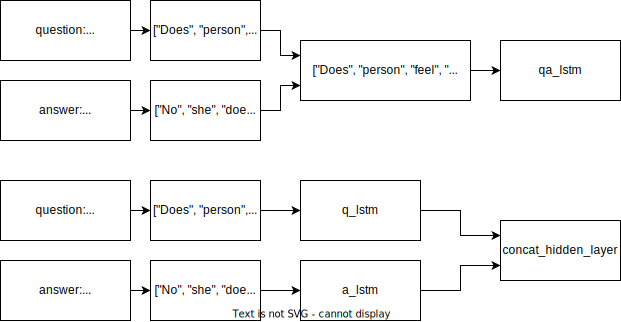
\includegraphics[width=.55\textwidth,keepaspectratio]{content/chapters/methodology/model_adaptation/figures/concat lstms vs q and a lstms.jpg}
    \captionsource(How Q and A are fed into the model){The difference in structure between the original (above) intended method --- where both question and answer are concatenated together --- and the final (below) method --- where the question and answer are passed into separate \glspl{lstm}.}{Original diagram prepared for this dissertation}
\end{figure}

%  Add a diagram explaining the changes made (such as a before and after).
% It needs to clearly illustrate the difference in structure between the original and the new implementation.

% Explain the training process (loading of data, initialisation of model, splitting of question and answer into pairs, setting of 0 or 1 if answer is correct, etc.)


\clearpage
\section{Experiments}
\label{sec:experiments}

Several experiments were conducted on the model to evaluate its performance on \gls{vcr}.
The experiments were designed to test the models accuracy over the three main task types (Q\rightarrow{}A, QA\rightarrow{}R, Q\rightarrow{}AR) discussed in Section~\ref{subsec:vcr_dataset} using different word embedding approaches and input encoder configurations.
Combinations of task type, \gls{bilstm} configuration in the model input unit and input token embedding types (contextual and noncontextual) were chosen as experiments to target what factors improve performance and what task types see the biggest improvement in prediction accuracy.

An additional experiment was also conducted on QA\rightarrow{}R to determine how big an influence the input answers had on the predicted rationale, and whether using previously-predicted answers as input would result in a significant drop in accuracy.
To test this, the model was first trained to predict the correct answers in Q\rightarrow{}A mode, exporting the predicted answers to a prediction file.
Then a new model was trained in QA\rightarrow{}R mode, using the predicted correct answers instead of the true correct answers.

\subsection{Setup}
\label{subsec:experiment-setup}

The model was trained on a single machine node with up to two \acrshort{gpu} nodes to use, depending on the configuration used for each experiment.
Each model was trained using a configuration file that selected the hyper-parameters used and task type to be tested.
To keep track of the model training history, model checkpoints were taken during training after every predefined number of steps.
Training was performed up to the specified step count, after which the model was evaluated using each of the recorded checkpoints.
To avoid recording the performance of an overfit model, the model performance chosen was taken from the step with the highest accuracy and not the most recent step.

\subsection{Ablations}
\label{subsec:experiment-ablations}

A set of ablation experiments were developed as part of the main experiments to determine the accuracy contribution of various components of the model.
Namely, those experiments deciding embedding types and \gls{bilstm} configuration.

The ablation tested is the use of context-aware token embeddings over context-free token embeddings, and whether a higher embedding dimensionality contributes to improved performance or not.
For this, BERT was chosen as the sentence-level context-aware embedding, retaining the same embeddings published by \citeauthor{zellers_recognition_2019} alongside the \gls{vcr} dataset and their \gls{r2c} model\cite{zellers_recognition_2019}.
To test context-free embeddings, GLOVE is used since it is the same embedding scheme used by \gls{snmn} and \gls{n2nmn} in their training and evaluation.
As an additional measure in testing context-free embeddings, Word2Vec embeddings are used which are generated using a Continuous Bag-Of-Words model\cite{mikolov_we_2013}.
Two sets of Word2Vec embeddings are generated, one with 300-dimensional vectors to match the GLOVE dimensionality and one with 768-dimensional vectors to match the BERT vectors.
This will both determine how big an effect both vector dimensionality and sentence-level context have on accuracy.

Another ablation is the testing of how the model input unit encodes the input sentences.
Seeing as the original model was designed with only a single token sequence in mind, one \gls{bilstm} encodes the sequence, but since we have more than one sequence as input, multiple \glspl{bilstm} are needed to encode each sequence.
As an ablation, another experiment is conducted where the model uses a single \gls{bilstm} to encode all three sequences.
This evaluates whether a single \gls{bilstm} would bottleneck the layout generation or improve it.


\chapter{Experiments}
\label{chp:experiments}

Several experiments were conducted on the model to evaluate its performance on \gls{vcr}.
The experiments were designed to test the models accuracy across the 3 main task types discussed in \ref{subsec:vcr_dataset} using different word embedding approaches and input encoder configurations.
Combinations of task type, \gls{lstm} configuration in the model input unit and input token embedding types (contextual and noncontextual) were chosen as experiments to target what factors improve performance and what task types see the most improvement.

An additional experiment was also conducted on QA \rightarrow R to determine how big an influence answers had on the predicted rationale.
The model was first trained to predict the correct answers in Q \rightarrow A mode, exporting the predicted answers to a prediction file.
Then a new model was trained in QA \rightarrow R mode, using the predicted correct answers instead of the true correct answers.

\section{Setup}
\label{sec:experiment-setup}

The model was trained on a single machine node with up to two \acrshort{gpu} nodes to use, depending on the configuration used for each experiment.
Each model was trained using a configuration file that selected the hyper-parameters used and task type to be tested.
To keep track of the model training history, model checkpoints were taken during training after every predefined number of steps.
Training was performed up to the specified step count, after which the model was evaluated using the recorded checkpoints.
To avoid recording the performance of an overfit model, the model performance chosen was taken from the step with the highest accuracy and not the most recent step.

\section{Challenges}
\label{sec:experiment-challenges}

Several errors were encountered during training.
The most common error encountered was unstable learning which resulted in NaN loss errors or slow learning.
NaN losses were frequent when training the model using word2vec embeddings and didn't occur at all when using glove or bert.
Slow learning rates were observed during glove and word2vec training, especially with Q \rightarrow AR training.
Another factor in getting good predictions was batch size, which was strained by the task size and amount of data involved.
To work around the limited batch size available, training on QA \rightarrow R and Q \rightarrow AR modes was performed on a multi-gpu setup to allow for increased batch size.
This setup produced better learning rates and prediction performance compared to single-gpu training.

\section{Evaluation results}
\label{sec:evaluation-results}

Something

\begin{table}
\centering

\begin{tabular}{| l | l | l | l | l | l | l | l |}
\hline
 & Q->A

Shared LSTM & Q->A

Separate LSTMs & QA->R

Shared LSTM & QA->R

Separate LSTMs & QA->R

Shared LSTM (With predicted answers) & Q->AR

shared & Q->AR

Separate LSTMs \\
\hline
Glove & 52\textsuperscript{[1]} & 51\textsuperscript{[1]} & 25& 47\textsuperscript{[7]} &  & 6.4 & 6.4\textsuperscript{[1][7]} \\
\hline
BERT & 63\textsuperscript{[1]} & 63\textsuperscript{[1]} & 60\textsuperscript{[1][7]} & 60\textsuperscript{[7]} & 60\textsuperscript{[7][8]} & 24.7 & 24 \\
\hline
w2v-300 & 33\textsuperscript{[2]} & 34\textsuperscript{[6]} & 25& 32\textsuperscript{[1][6][7]} &  &  &  \\
\hline
w2v-768 & 32\textsuperscript{[2]} & 34 & 25& 32\textsuperscript{[7]} &  &  &  \\
\hline

\end{tabular}

\end{table}




\printbibliography[title=References]

\appendix{}

\chapter{Sample A}

Lorem ipsum dolor sit amet, consectetur adipiscing elit.
Mauris sed ipsum risus.
Nulla aliquet quis quam sed eleifend.
Donec rutrum, dolor id vulputate pharetra, nulla tortor laoreet nisl,
pellentesque dapibus velit dolor suscipit purus.
Phasellus vitae eleifend sem.
Integer ultricies ex in neque pellentesque, vitae facilisis orci aliquam.
In pellentesque mollis turpis, eu tristique lacus eleifend nec.
Vestibulum orci neque, rhoncus vitae convallis eu, suscipit quis dui.
Nulla libero elit, porta sit amet sagittis vel, placerat sit amet tortor.
Aliquam hendrerit dolor sit amet sollicitudin ornare.
Aliquam placerat sodales est, in vestibulum nisl efficitur in.
Nulla venenatis aliquam sem, at volutpat nisl pellentesque eleifend.
Praesent vitae euismod nulla, eget vehicula turpis.
Duis quis tellus vitae nisi tempus tincidunt.

Nam quis aliquet nisi, non pharetra ligula.
Phasellus pulvinar mattis neque, nec interdum justo condimentum hendrerit.
Mauris fermentum venenatis faucibus.
Pellentesque egestas eleifend libero, quis placerat ante fermentum et.
Suspendisse accumsan gravida rhoncus.
Vestibulum auctor sodales vehicula.
Pellentesque a urna et elit placerat laoreet a quis turpis.
Morbi ut sem at nunc posuere malesuada vel nec libero.
Nam et urna suscipit, bibendum diam sed, aliquet leo.
Lorem ipsum dolor sit amet, consectetur adipiscing elit.
Ut pretium mauris et nulla malesuada, mattis tristique lectus molestie.
Aenean accumsan iaculis quam, eget varius libero placerat eu.
Fusce mauris justo, vulputate a sollicitudin a, malesuada at est.
Sed ac augue elit.
Maecenas massa lorem, tincidunt vitae neque et, maximus dictum tellus.

% \chapter{Sample A}

Lorem ipsum dolor sit amet, consectetur adipiscing elit.
Mauris sed ipsum risus.
Nulla aliquet quis quam sed eleifend.
Donec rutrum, dolor id vulputate pharetra, nulla tortor laoreet nisl,
pellentesque dapibus velit dolor suscipit purus.
Phasellus vitae eleifend sem.
Integer ultricies ex in neque pellentesque, vitae facilisis orci aliquam.
In pellentesque mollis turpis, eu tristique lacus eleifend nec.
Vestibulum orci neque, rhoncus vitae convallis eu, suscipit quis dui.
Nulla libero elit, porta sit amet sagittis vel, placerat sit amet tortor.
Aliquam hendrerit dolor sit amet sollicitudin ornare.
Aliquam placerat sodales est, in vestibulum nisl efficitur in.
Nulla venenatis aliquam sem, at volutpat nisl pellentesque eleifend.
Praesent vitae euismod nulla, eget vehicula turpis.
Duis quis tellus vitae nisi tempus tincidunt.

Nam quis aliquet nisi, non pharetra ligula.
Phasellus pulvinar mattis neque, nec interdum justo condimentum hendrerit.
Mauris fermentum venenatis faucibus.
Pellentesque egestas eleifend libero, quis placerat ante fermentum et.
Suspendisse accumsan gravida rhoncus.
Vestibulum auctor sodales vehicula.
Pellentesque a urna et elit placerat laoreet a quis turpis.
Morbi ut sem at nunc posuere malesuada vel nec libero.
Nam et urna suscipit, bibendum diam sed, aliquet leo.
Lorem ipsum dolor sit amet, consectetur adipiscing elit.
Ut pretium mauris et nulla malesuada, mattis tristique lectus molestie.
Aenean accumsan iaculis quam, eget varius libero placerat eu.
Fusce mauris justo, vulputate a sollicitudin a, malesuada at est.
Sed ac augue elit.
Maecenas massa lorem, tincidunt vitae neque et, maximus dictum tellus.

% \input{content/appendices/examples/appendix_b}

\end{document}
